\documentclass[12pt]{article}

\newif\ifpdf
\ifx\pdfoutput\undefined
\pdffalse % not running PDFLaTeX
\else
\pdfoutput=1 % running PDFLaTeX
\pdftrue
\fi

\ifpdf
\usepackage[pdftex]{graphicx}
\else
\usepackage{graphicx}
\fi

%\usepackage[osf]{gtamachoefler}

% Added by bcarey
% Bibliography support
\usepackage{lscape}
\usepackage[super,comma,sort]{natbib}
%\usepackage[linux]{vpe}
%\vpesetup{noref}
%define citation punctuation style
\bibpunct[, ]{(}{)}{;}{a}{,}{,}

% Allow less text and more figure on page
\renewcommand{\topfraction}{0.90}
\renewcommand{\bottomfraction}{0.90}
\renewcommand{\textfraction}{0.1}
\renewcommand{\floatpagefraction}{0.90}

% end additions by bcarey


%\usepackage{times}
\usepackage{fourier}
\usepackage{sectsty,hangcaption}
\usepackage{amsmath,amsbsy,amssymb}
%\usepackage{deflist}
\usepackage{fancyhdr}
\usepackage{tabularx}
\usepackage{verbatim}
\usepackage{moreverb}
\usepackage{float}
\usepackage{fancybox}
\usepackage{graphicx}
\usepackage{longtable}
\usepackage{wrapfig}
\usepackage{booktabs}
\usepackage{comment}
%\usepackage{subfigure}

%must be last package
%\usepackage{hyperref}
\usepackage[debug=false, colorlinks=true, pdfstartview=FitV, linkcolor=blue, citecolor=blue, urlcolor=blue]{hyperref}

%\usepackage{toc_entr}
\textwidth 6.5in
\textheight 9.in
%\topmargin -0.75in
\topmargin -0.25in
%\topmargin -3.280cm
\newlength{\boxwidth}
\setlength{\boxwidth}{5.8in}
\oddsidemargin 0in
\evensidemargin 0in
\headheight 0.25in
\renewcommand{\thepage}{\arabic{section}--\arabic{page}}
%\lhead{ }
\lhead{}
\rhead{\today}
\chead{}
\cfoot{[\thepage]}
\lfoot{}
\rfoot{}
%\footrulewidth 0.4pt
\newcommand{\negsp}{\vspace{-4mm}}
\newcommand\secsp{\vspace{-3 mm}}
\newcommand\secspb{\vspace{-2 mm}}
\newcommand\subsecsp{\vspace{-0.0 mm}}
\renewcommand{\baselinestretch}{.9}
%\setlength{\baselineskip}{13pt}
\def\EQ#1\EN{\begin{equation}#1\end{equation}}
\def\BA#1\EA{\begin{align}#1\end{align}}
\def\BS#1\ES{\begin{split}#1\end{split}}
%\newcommand{\EQ}{\begin{equation}}
%\newcommand{\EN}{\end{equation}}
\newcommand{\longline}{\noindent\rule[-0.1in]{\textwidth}{0.01in}}
\newcommand{\bc}{\begin{center}}
\newcommand{\ec}{\end{center}}
\newcommand{\degc}{$^\circ$C}
\newcommand{\eq}{\ =\ }
\newcommand{\eff}{{\rm eff}}
\newcommand{\eqr}{{\rm le}}
\newcommand{\equ}{{\rm eq}}
\newcommand{\kin}{{\rm kin}}
\newcommand{\rdx}{{\rm rdx}}
\newcommand{\ind}{{\rm id}}
\newcommand{\dep}{{\rm dp}}
\newcommand{\e}{{\rm{e}}}
\newcommand{\erf}{{\rm{erf}}}
\newcommand{\erfc}{{\rm{erfc}}}
\newcommand{\sign}{{\rm{sign}}}
\newcommand{\p}{{\partial}}
\newcommand{\A}{{\mathcal A}}
\newcommand{\B}{{\mathcal B}}
\newcommand{\C}{{\mathcal C}}
\newcommand{\D}{{\mathcal D}}
\newcommand{\E}{{\mathcal E}}
\newcommand{\F}{{\mathcal F}}
\newcommand{\G}{{\mathcal G}}
\renewcommand{\H}{{\mathcal H}}
\newcommand{\I}{{\mathcal I}}
\newcommand{\J}{{\mathcal J}}
\newcommand{\jo}{{j_o}}
\newcommand{\M}{{\mathcal M}}
\newcommand{\cO}{{\mathcal O}}
\renewcommand{\P}{{{\mathcal P}}}
\newcommand{\Q}{{\mathcal Q}}
\newcommand{\R}{{{\mathcal R}}}
\renewcommand{\S}{{\mathcal S}}
\newcommand{\T}{{\mathcal T}}
\newcommand{\W}{{\mathcal W}}
\newcommand{\X}{{\mathcal X}}
\newcommand{\Y}{{\mathcal Y}}
\newcommand{\Z}{{\mathcal Z}}
\newcommand{\rev}{{\rm rev}}
\newcommand{\irr}{{\rm irr}}
\renewcommand{\a}{{\alpha}}
\newcommand{\abar}{{\bar \alpha}}
\renewcommand{\b}{{\beta}}
\newcommand{\w}{{\rm H_2O}}
\newcommand{\air}{{\rm N_2}}
\newcommand{\pe}{{\rm Pe}}
\newcommand{\da}{{\rm Da}}
\renewcommand{\k}{{\dot R}^0}
\renewcommand{\L}{\widehat{\mathcal L}}
\renewcommand{\bar}{\overline}
\newcommand{\dsty}{{\displaystyle}}
\newcommand{\diff}{{\mathcal D}}
\newcommand{\surf}{\equiv \!\!\!}
\newcommand{\bnabla}{\boldsymbol{\nabla}}
\newcommand{\bA}{\boldsymbol{A}}
\newcommand{\ba}{\boldsymbol{a}}
\newcommand{\bB}{\boldsymbol{B}}
\newcommand{\bC}{\boldsymbol{C}}
\newcommand{\bD}{\boldsymbol{D}}
\newcommand{\bE}{\boldsymbol{E}}
\newcommand{\bF}{\boldsymbol{F}}
\newcommand{\bi}{\boldsymbol{i}}
\newcommand{\bI}{\boldsymbol{I}}
\newcommand{\bJ}{\boldsymbol{J}}
\newcommand{\bK}{\boldsymbol{K}}
\newcommand{\blambda}{\boldsymbol{\lambda}}
\newcommand{\bM}{\boldsymbol{M}}
\newcommand{\bg}{\boldsymbol{g}}
\newcommand{\bGamma}{\boldsymbol{\Gamma}}
\newcommand{\bOmega}{\boldsymbol{\Omega}}
\newcommand{\bPsi}{\boldsymbol{\Psi}}
\newcommand{\bO}{\boldsymbol{O}}
\newcommand{\bnu}{\boldsymbol{\nu}}
\newcommand{\bdS}{\boldsymbol{dS}}
\newcommand{\bq}{\boldsymbol{q}}
\newcommand{\br}{\boldsymbol{r}}
\newcommand{\bR}{\boldsymbol{R}}
\newcommand{\bS}{\boldsymbol{S}}
\newcommand{\bu}{\boldsymbol{u}}
\newcommand{\bv}{\boldsymbol{v}}
\newcommand{\bz}{\boldsymbol{z}}
\newcommand{\arrows}{~\rightleftharpoons~}
\newcommand{\arrowstab}{\!\!\!\rightleftharpoons\!\!\!}
\newcommand{\CA}{C_{\rm A}}
\newcommand{\CB}{C_{\rm B}}
\newcommand{\CC}{C_{\rm C}}
\newcommand{\CAB}{C_{\rm AB}}
\newcommand{\CBC}{C_{\rm BC}}
\newcommand{\RA}{\R_{\rm A}}
\newcommand{\RB}{\R_{\rm B}}
\newcommand{\RC}{\R_{\rm C}}
\newcommand{\RAB}{\R_{\rm AB}}
\newcommand{\RBC}{\R_{\rm BC}}
%\newcommand{\kdsc}{K^{DS}}
%\newcommand{\kdec}{K^{DE}}
%\newcommand{\kdsm}{\overline K^{DS}}
%\newcommand{\kdem}{\overline K^{DE}}
\newcommand{\kdsc}{K^{sc}}
\newcommand{\kdec}{K^{ec}}
\newcommand{\kdsm}{K^{sm}}
\newcommand{\kdem}{K^{em}}
\newcommand{\csm}{S}
\renewcommand{\csc}{S}
\newcommand{\cem}{\E}
\newcommand{\cec}{\E}
\renewcommand{\min}{{\rm min}}
\newcommand{\coll}{{\rm coll}}
\newcommand{\ex}{{\rm ex}}
\newcommand{\srf}{{\rm sc}}
\def\dbar{{\mkern2mu\mathchar'26\mkern-11mu\mathrm{d}}}

\newcounter{saveeqn}%
\newcommand{\alpheqn}{\setcounter{saveeqn}{\value{equation}}%
\stepcounter{saveeqn}\setcounter{equation}{0}%
\renewcommand{\theequation}
      {\mbox{\arabic{saveeqn}\alph{equation}}}}%
\newcommand{\reseteqn}{\setcounter{equation}{\value{saveeqn}}%
\renewcommand{\theequation}{\arabic{equation}}}%

\renewcommand{\contentsname}{Table of Contents}
\renewcommand{\listfigurename}{{List of Figures}}
\renewcommand{\listtablename}{{List of Tables}}

\renewcommand{\arraystretch}{1.3}

\setlength{\parindent}{0.3125in}
\setlength{\parskip}{2ex plus 0.2ex minus 0.2ex}

\setcounter{secnumdepth}{5}
\setcounter{tocdepth}{5}

\pagestyle{fancy}

\thispagestyle{empty}

%\renewcommand{\theequation}{\arabic{section}.\arabic{equation}}
%\renewcommand{\thetable}{{\arabic{section}.\arabic{table}}}
%\renewcommand{\thefigure}{{\arabic{section}.\arabic{figure}}}

\begin{document}


\subsection*{Conceptual Design of PETSc Time Stepper for Flow and Transport}
\addcontentsline{toc}{section}{Background}
\vspace{-16pt}
~
The generalized partial differential equation for groundwater flow is 
\begin{equation}\label{flow}
\frac{\p}{\p t} \varphi\rho + \bnabla\cdot\rho\bu\eq \S,
\end{equation}
with $\bu$ given by Darcy's law
\begin{equation}
\bu\eq-\frac{\kappa}{\mu}\nabla\big(p-W\rho g z\big),
\end{equation}
with permeability $\kappa$, viscosity $\mu$, molar fluid density $\rho$, formula weight of water $W$, acceleration of gravity $g$, and source/sink term $\S$. For reactive solute transport, the generalized partial differential equation takes the form
\begin{equation}\label{tran}
\frac{\p A}{\p t} + \bnabla\cdot\bF \eq \S,
\end{equation}
with accumulation term $A$, source/sink term $\S$, and flux term $\bF$ of the form
\begin{equation}
\bF \eq \bu\rho X - \phi D \rho\bnabla X.
\end{equation}
Although these two equations are coupled through the Darcy flow velocity $\bu$, and could be solved simultaneously, the equations are usually loosely-coupled and solved sequentially since the flow time scales are generally larger than transport time scales.  With both flow or transport, time steps are generally small at the beginning of a simulation and grow to some maximum time step size, which is governed by either convergence or stability/accuracy criterion. During a flow or transport simulation, time steps are often cut due to (1) a lack of convergence, (2) transient boundary conditions or source/sinks, (3) reporting criteria (print data $X$ at time $T$). Therefore, time stepping within PFLOTRAN must be extremely flexible based on any of the 3 criterion above.  

One way to view time stepping is to take a waypoint approach such as that used in autonomous flight.  The pilot programs waypoints into the flight plan.  The aircraft flies to each waypoint, increments its instruction set, and flies to the next waypoint. With numerical modeling, waypoints can be set based on transient boundary conditions and source/sinks and reporting requirements.  Upon model initialization, a linked list of waypoints is constructed for all time varied phenomenon within the simulation (e.g. transient sources, I/O, etc.).  During the simulation, the model then traverses that list updating processes and performing I/O as necessary. In order to traverse such a waypoint list, time stepping must be flexible.  For instance, suppose that the simulation time and time step are 9.8 and 0.5, respectively, and waypoints exist at 10.0 (e.g. change in boundary condition) and 10.25 (e.g. I/O).  The time stepper must reduce the time step to 0.2 to hit the waypoint at 10.0, and then increase the time step to 0.25 for I/O, as shown in Figure \ref{timeline}.  Assuming no other waypoints exist between 10.25 and 10.75, the time stepper would ideally set the time step back to 0.5 after passing the waypoint at 10.25.

\begin{figure}[h]\centering
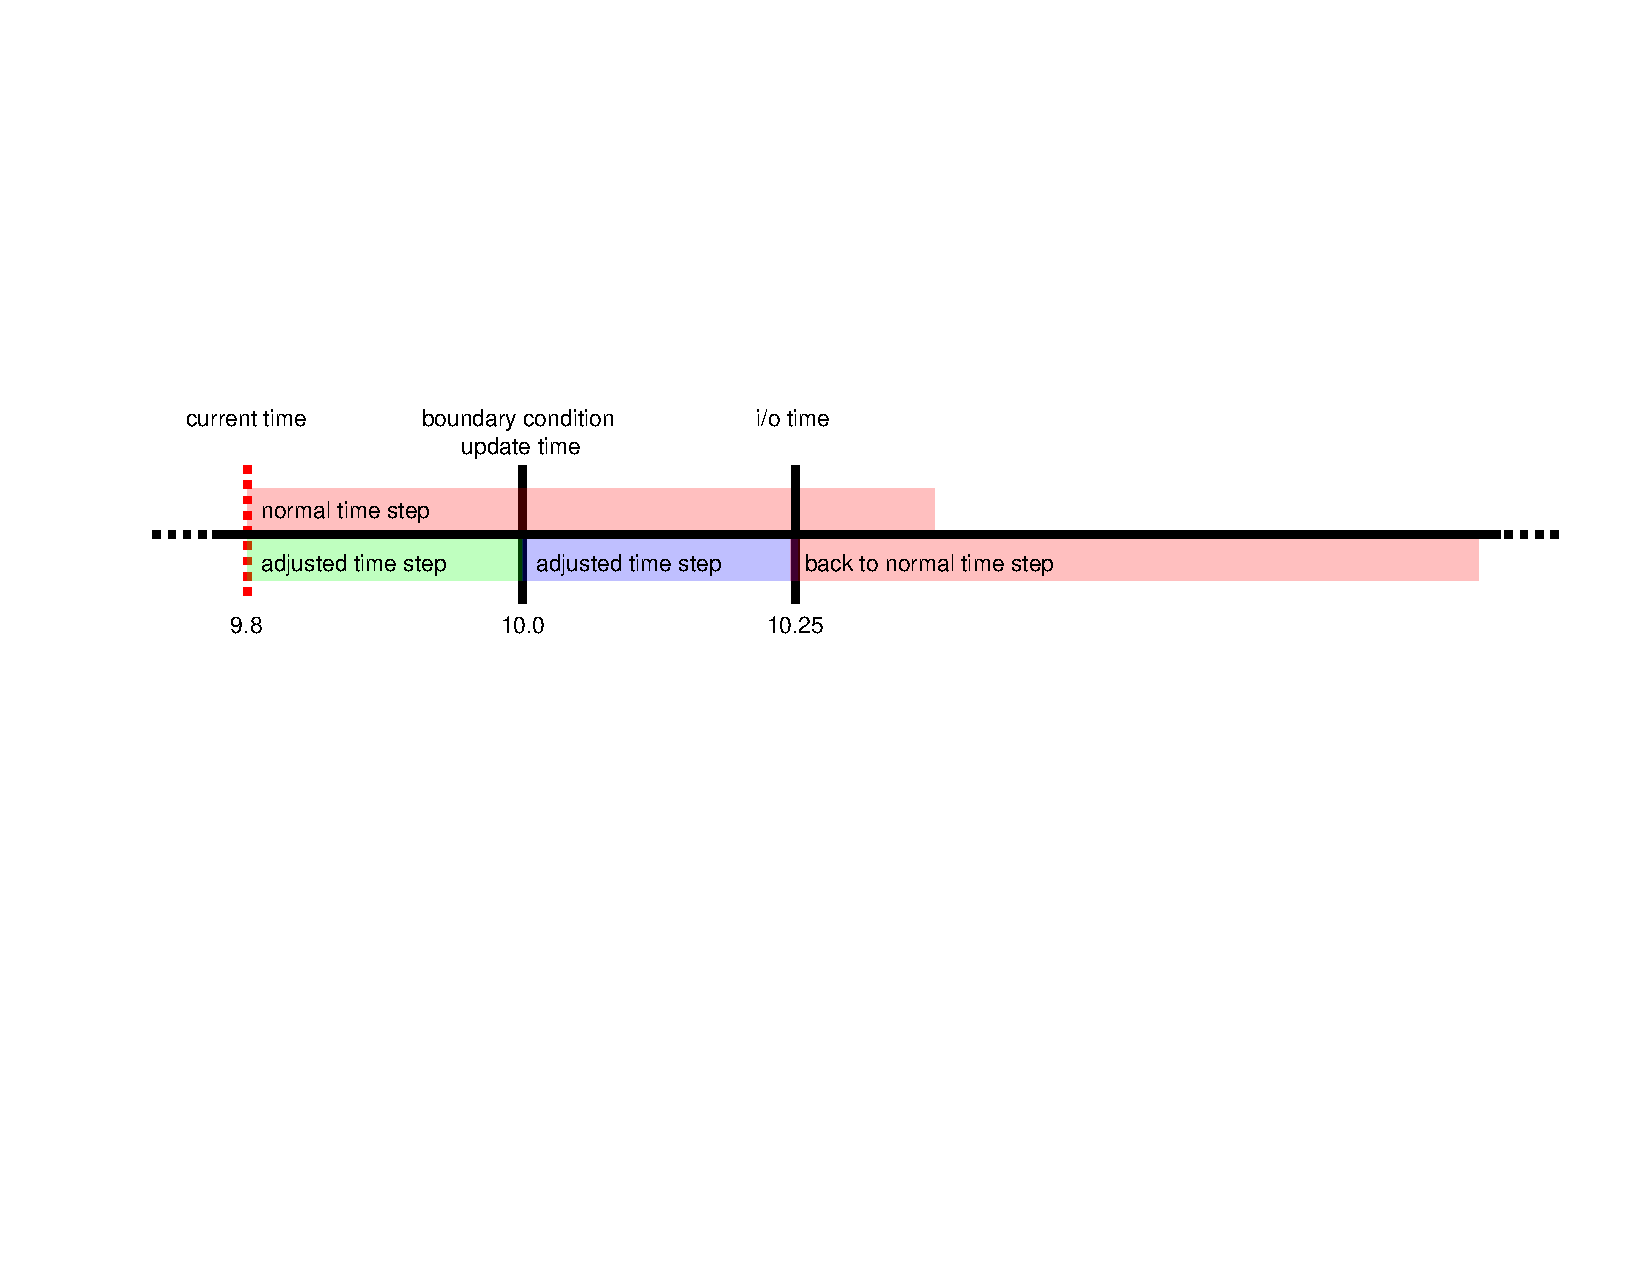
\includegraphics[width=6.0in]{./figs/timeline}
\caption{Adjustment of time step size to accommodate waypoints in simulation.}\label{timeline}
\end{figure}

Another complication is the alignment of flow and transport.  Although not always the case, transport time steps are generally smaller than flow time steps due to Courant criteria.  A simple approach to synchronizing flow and transport times steps would be setting the time step for both flow and transport equal to the limiting time step size, most often transport.  For instance, suppose in the case of mineral dissolution that the transport model exits quasi-stationary state due to the depletion of mineral within a cell.  For large time steps sizes, this somewhat drastic change in the state of the model results in an inability to converge unless step step size is reduced.  Thus, the transport solver would cut the time step size for both flow and transport and both solutions would be recomputed at the new time step size.  Clearly, this approach would result in excessive computation, since the model may continue to cut the time step until it is sufficiently small for convergence, and all this time the flow solution is being recomputed.

Perhaps a better approach is to allow the larger flow time steps to proceed on their own, and within each flow time step take multiple transport time steps as shown in Figure \ref{ts_align}.  A transport waypoint is then set at the end of flow time step, simply to align the time steps.

\begin{figure}[h]\centering
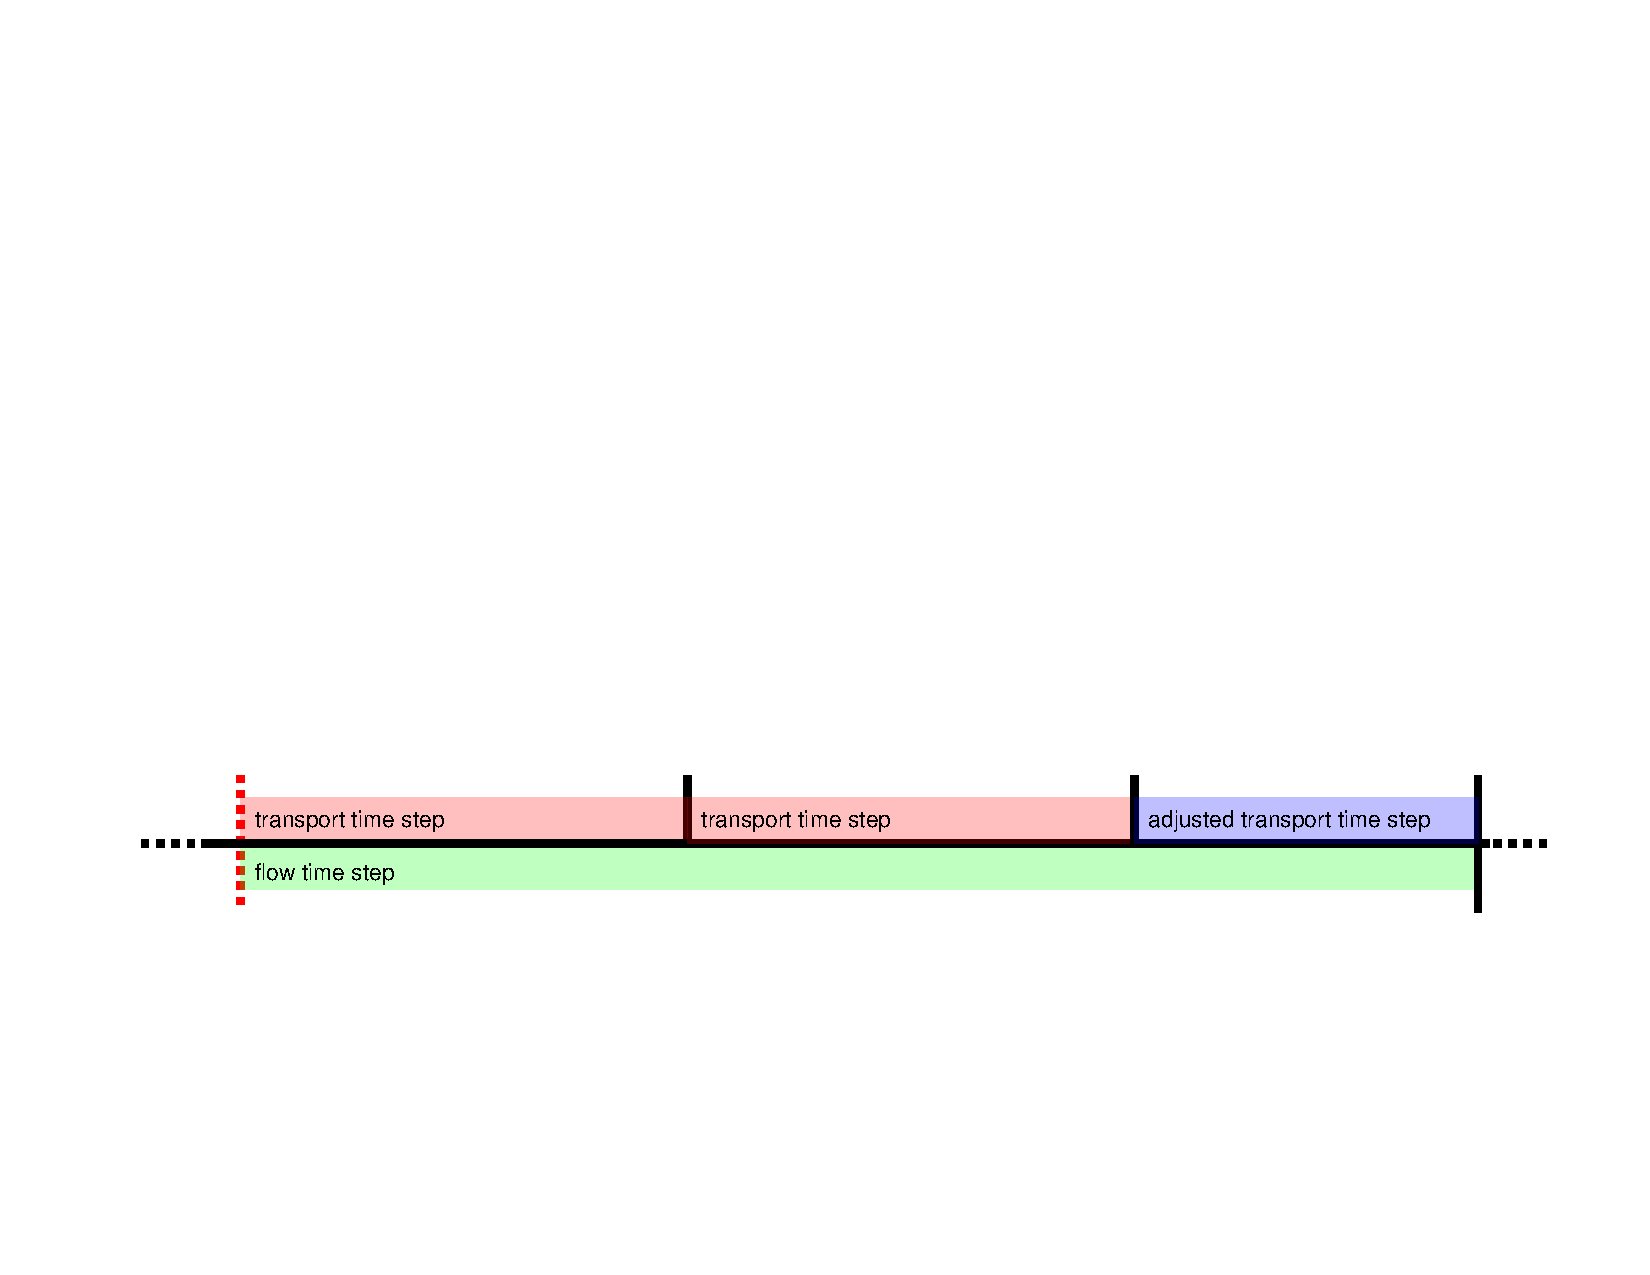
\includegraphics[width=6.0in]{./figs/ts_alignment}
\caption{Adjustment of time step size to accommodate waypoints in simulation.}\label{ts_align}
\end{figure}
\end{document}
